\section{Security and privacy}
\label{sec:security-privacy}

Privacy is a design property of Meowtion, not a setting bolted on afterwards. The strongest guarantees
come from where work happens (on the collar) and how data is scoped (per owner, by enforced rules).

\subsection{On-device audio}

The microphone is used only for on-device classification. Audio is processed on the collar and
discarded; it is never written to flash in normal operation and never transmitted in production mode.
The collar's uplink is a classification result (a class index and a confidence), not a sensor stream.
The one exception is deliberate and owner-driven: in training mode the owner chooses to capture clips
to teach a behaviour, and those clips are stored privately to their own account and are never
world-readable, even for the public demo.

\subsection{Per-owner isolation}

All of an owner's data lives under \texttt{users/<uid>/}, and the database and storage rules scope
every read and write to the owning account, so owners (and their token-authenticated devices) touch
only their own data. Isolation is enforced by the backend, not the client. The Storage rules go
further and deny \emph{all} direct client writes: training clips are written only by the
\texttt{upload\_clip} function and are readable only by their owning account, and model blobs are
public-read (so the token-only station can fetch one) but writable only by the trainer.

\subsection{Device tokens, not credentials}

A station authenticates with a scoped, revocable per-device token rather than the owner's password, and
a collar holds nothing at all. A lost or compromised device therefore cannot expose the owner's
credentials, and it can be revoked simply by deleting its token from the account, with no password
change and no effect on the owner's other devices. The token is carried in an \texttt{Authorization}
header rather than a URL or query string, so it stays out of request logs, and the rules let an account
claim only an unclaimed token or one it already owns, so a known token cannot be re-pointed to another
account. \Cref{fig:token} traces the token's lifecycle.

\begin{figure}[ht]\centering
  \begin{tikzpicture}[node distance=10mm and 14mm, every node/.style={font=\footnotesize}]
    \node[mwterm] (mint) {Dashboard mints token T\\\scriptsize records \texttt{deviceTokens/T/owner}};
    \node[mwflow, below=of mint, text width=6.6cm, align=left] (store)
      {Station stores T in NVS and presents it on every cloud request (no login)};
    \node[mwflow, below=15mm of store, xshift=-26mm, text width=4cm, align=left] (rules)
      {Database rules: T maps to the owner, so writes to that owner's subtree are allowed};
    \node[mwflow, below=15mm of store, xshift=26mm, text width=4cm, align=left] (upl)
      {\texttt{upload\_clip} verifies T's owner and writes the clip as admin};
    \node[mwterm, below=38mm of store] (revoke) {Revoke: delete the token; all its access is denied};
    \draw[mwedge] (mint) -- (store);
    \draw[mwedge] (store) -- (rules);
    \draw[mwedge] (store) -- (upl);
    \draw[mwedge] (rules) -- (revoke);
    \draw[mwedge] (upl) -- (revoke);
  \end{tikzpicture}
  \caption{Credential-token lifecycle. A device is minted a scoped token that maps to its owner; the
           token authorises database writes and clip uploads, and deleting it revokes the device.}
  \label{fig:token}
\end{figure}

\subsection{Enforced read-only demo}

The public demo reads a single designated demo account's data, which the rules make world-readable, but
that account is write-locked at the backend: the demo cannot change any data or trigger any function.
The read-only behaviour is enforced by the rules, not merely hidden in the interface, so it holds even
against a hand-crafted client.

\subsection{Secret handling}

The Firebase web API key shipped in the static front end is a public client identifier, not a secret;
security is enforced by Authentication and the rules, not by hiding the key. No service-account key is
present in the repository, and the functions run on their ambient service account. Device Wi-Fi
credentials are entered at runtime and never committed, and \texttt{.gitignore} guards against any
local secret file. Everything required to understand and build the system is tracked; only true
secrets are not.

\subsection{Independent security audit}

The codebase is checked automatically as well as by hand. Every push and pull request runs CodeQL
static analysis, and dependency updates are raised automatically. In addition the repository was put
through an independent third-party static audit (Aikido), which reads the firmware, the cloud rules and
the application code and reasons about attacker-reachable paths. \Cref{fig:aikido} shows that audit as
first reported.

\begin{figure}[ht]\centering
  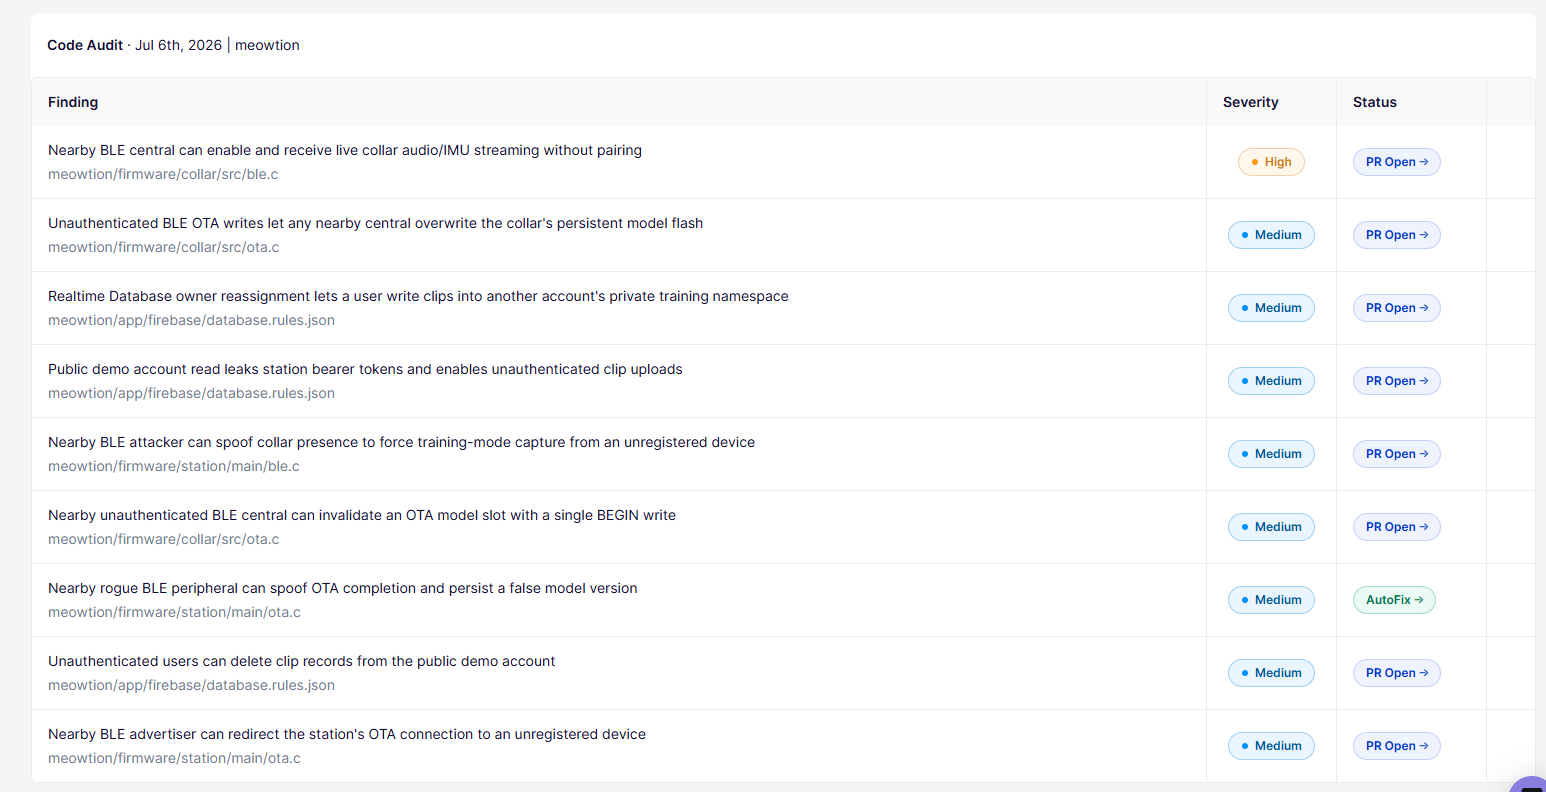
\includegraphics[width=\textwidth]{aikido-scan.png}
  \caption{Independent static application-security audit of the repository. Each finding was reviewed
           against the running system and dispositioned in \cref{tab:audit-triage}.}
  \label{fig:aikido}
\end{figure}

Each finding was triaged against the actual design rather than accepted blindly, because an
auto-generated patch can break a working device: the base station authenticates to the backend with a
scoped device token and no interactive login. Several of the proposed fixes, checked in review, would
have done exactly that: requiring a Firebase login on the device write path rejects every telemetry
write from the token-only station, and adding encryption to the collar alone drops the connection from a
station that does not pair. The fixes were therefore reworked to keep the system running, and the BLE
link was then encrypted properly, on both MCUs at once. \Cref{tab:audit-triage} records the disposition
of each finding.

\begin{table}[ht]
  \centering
  \caption{Audit findings and their disposition.}
  \label{tab:audit-triage}
  \begin{tabularx}{\textwidth}{@{}X l X@{}}
    \toprule
    \textbf{Finding} & \textbf{Sev.} & \textbf{Disposition} \\
    \midrule
    Realtime Database token owner could be reassigned & Med &
      \textbf{Fixed.} The \texttt{deviceTokens} write rule now pins an existing token's owner, so a
      registered token cannot be re-pointed at another account; creation and revocation are unaffected. \\
    Device write path takes no interactive login & Med &
      \textbf{By design.} The per-device token is the capability: scoped, revocable and carried in the
      \texttt{Authorization} header (\cref{fig:token}). A login is required on the human write path;
      requiring one on the device path would break the token-only station by design. \\
    Public demo read exposure & Med &
      \textbf{Reviewed.} The demo-readable subtree carries activity data only, never a device token, and
      the demo account is write-locked at the backend, so nothing sensitive is reachable through it. \\
    Nearby device could spoof presence to force training capture & Med &
      \textbf{Mitigated.} Training capture runs only for a collar on the station's registration
      allow-list ($\texttt{g\_allow}$); an unregistered advertiser cannot trigger it. \\
    Nearby device could stream audio, write an OTA model, or spoof an OTA version over BLE & High / Med &
      \textbf{Fixed.} The collar-to-station link now requires an encrypted connection (LE Secure
      Connections, with a fresh key agreement per connection so no stale pairing state accumulates on a
      battery device that reboots often). An unpaired device can no longer subscribe to the audio stream
      or write an OTA model, so it can neither eavesdrop nor overwrite the model flash; an OTA image is in
      any case committed only after a CRC-32 integrity check (\cref{sec:training-pipeline}). Authenticating
      the pairing against an active man-in-the-middle, with a key provisioned over USB, is future work
      (\cref{sec:future-work}). \\
    \bottomrule
  \end{tabularx}
\end{table}

The residual item is authenticating that encrypted local link against an active man-in-the-middle, which
is future work; the link is already encrypted, and the boundary that matters, the cloud where the data
actually lives, is closed by Authentication and the rules above.

\subsection{Owner data rights}

The account page lets an owner export everything stored about their cats and delete their account,
devices, and data. This supports the access and erasure expectations of data-protection regimes such as
the UK GDPR. The bundled privacy policy is a starting point and is marked for legal review before any
public launch.
